% !TEX root = frenetic_programmers_guide.tex

\chapter{Quick Start}

In this book, you will use Frenetic to create a full-programmable network.  For the moment, let's assume you're familiar with Software Defined Networking and the OpenFlow protocol, and just dive right in.  (If you're not, don't worry!  We'll introduce some bedrock concepts in the next chapter and explain everything that happened here.)  

\section{Installation}

There are several ways to get started with Frenetic, but the easiest is to use Frenetic VM.  Frenetic itself only runs on Linux, but the Frenetic VM will run on any host system that supports VirtualBox, including Windows, Mac OS X and practically any version of Linux itself.   Keeping Frenetic it in its own VM will keep your own system clean and neat.  Later on, if you want to install Frenetic on a bare metal Ubuntu Linux server or network device, you can use the instructions in \ref{productionalizing:install}.  

\begin{itemize}
\item Install VirtualBox from https://www.virtualbox.org/wiki/Downloads.  Use the latest version platform package appropriate for your system.  
\item Install Vagrant at http://www.vagrantup.com/downloads.  Vagrant automates the process of building VM's from scratch, and Frenetic VM uses it to build its own environment.  This is more reliable than downloading a multi-gigabyte VM file.   
\item Install Frenetic VM from https://github.com/frenetic-lang/frenetic-vm.  You can simply use the Download Zip button and unzip to an appropriate directory on your system, like frenetic-vm.  Then from a terminal or command prompt:

\begin{lstlisting}[style=BashInputStyle]
 $ cd /path/to/frenetic-vm
 $ vagrant up
 ... lots of text 
\end{lstlisting}
\end{itemize}

The build process may take 15 minutes to an hour, depending on the speed of your system and Internet connection. 

\section{What Do You Get With Frenetic VM?}

At the end of the process you will have a working copy of Frenetic with lots of useful open source infrastructure:

\begin{description}
\item[Mininet] software builds a test network inside of Linux.  
It can simulate a topology with many switches and hosts.  
Writing a network application and throwing it into production is \ldots well, pretty risky, but running it on Mininet first can be a good test for how it works beforehand.  
We'll use it throughout this book.  
\item[Wireshark] captures and analyzes network traffic.  
It's a great debugging tool, and very necessary for sifting through large amounts of data.
\item[Frenetic].  This layer provides an easy-to-use programmable layer on top of ODL.  Its main job is to shuttle OpenFlow messages between ODL and your application, and to translate the language NetKAT into OpenFlow flow tables.  We'll see the differences between the two as we go.
\end{description}

Hmmm, that's a lot of software - what do {\it you} bring to the table?  You write your network application in Python, using the Frenetic framework.  As you'll see, it's quite easy to build a network device from scratch, and easy to grow it organically to fit your requirements.  Python is fairly popular, and knowing it will give you  a head start into Frenetic programming.  But if you're a Python novice that's OK.  As long as you know one object-oriented language fairly well, you should be able to follow the concepts.  We'll introduce you to useful Python features, like list comprehensions, as we go.  

\section{An Attempt at Hello World}

So let's dive right in.  We'll set up a Mininet network with one switch and two hosts.  First you should work from the directory where you installed Frenetic VM.

\begin{lstlisting}[style=BashInputStyle]
 $ cd /path/to/frenetic-vm
\end{lstlisting}
 
Then start up the VM:

\begin{lstlisting}[style=BashInputStyle]
 $ vagrant up
 ringing machine 'default' up with 'virtualbox' provider...
==> default: Clearing any previously set forwarded ports...
==> default: Clearing any previously set network interfaces...
==> default: Preparing network interfaces based on configuration...
    default: Adapter 1: nat
==> default: Forwarding ports...
    default: 22 => 2222 (adapter 1)
==> default: Running 'pre-boot' VM customizations...
==> default: Booting VM...
==> default: Waiting for machine to boot. This may take a few minutes...
    default: SSH address: 127.0.0.1:2222
    default: SSH username: vagrant
    default: SSH auth method: private key
    default: Warning: Connection timeout. Retrying...
==> default: Machine booted and ready!
==> default: Checking for guest additions in VM...
==> default: Setting hostname...
==> default: Mounting shared folders...
    default: /vagrant => /Users/cr396/frenetic-vm
    default: /home/vagrant/src => /Users/cr396/frenetic-vm/src
==> default: Machine already provisioned. Run `vagrant provision` or...
==> default: to force provisioning. Provisioners marked to run always...
\end{lstlisting}

Then log in to the VM.  At this point your command prompt will change to {\tt vagrant@frenetic} to distinguish it
from your host machine.

\begin{lstlisting}[style=BashInputStyle]
 $ vagrant ssh
Welcome to Ubuntu 14.04.2 LTS (GNU/Linux 3.16.0-30-generic x86_64)

 * Documentation:  https://help.ubuntu.com/
Last login: Tue Oct  6 10:35:06 2015 from 10.0.2.2
vagrant@frenetic:~$ 
\end{lstlisting}

So you are now working inside an Ubuntu-based VM.  You don't really need to know Ubuntu, but just know that Mac OS and Windows commands won't necessarily work here.  

Let's start up a Mininet network with one switch and two nodes.

\begin{lstlisting}[style=BashInputStyle]
vagrant@frenetic:~$ sudo mn --topo=single,2 --controller=remote
*** Creating network
*** Adding controller
Unable to contact the remote controller at 127.0.0.1:6633
*** Adding hosts:
h1 h2
*** Adding switches:
s1
*** Adding links:
(h1, s1) (h2, s1)
*** Configuring hosts
h1 h2
*** Starting controller
c0
*** Starting 1 switches
s1 ...
*** Starting CLI:
mininet>
\end{lstlisting}

The prompt changes to {\tt mininet>} to show your working in Mininet.  
The error message {\tt Unable to contact controller at 127.0.0.1:6633} looks a little ominous, but not fatal.  

You now have an experimental network with two hosts named h1 and h2.  
To see if there's connectivity between them, use the command \lstinline{h1 ping h2} which means ``On host h1, ping the host h2.''

\begin{lstlisting}[style=BashInputStyle]
mininet> h1 ping h2
PING 10.0.0.2 (10.0.0.2) 56(84) bytes of data.
From 10.0.0.1 icmp_seq=1 Destination Host Unreachable
From 10.0.0.1 icmp_seq=2 Destination Host Unreachable
From 10.0.0.1 icmp_seq=3 Destination Host Unreachable
^C
--- 10.0.0.2 ping statistics ---
6 packets transmitted, 0 received, +3 errors, 100\% packet loss, time 5014ms
pipe 3
\end{lstlisting}

The ping gets executed over and over again, but it's clearly not working.  So we press CTRL-C to stop and 
quit out of Mininet:

\begin{lstlisting}[style=BashInputStyle]
mininet> quit
\end{lstlisting}

So by default, hosts can't talk over the network to each other.  We're going to fix that by writing a {\it network
application}.    Frenetic will act as the controller on the network, and the network application tells Frenetic how to act.

\section{A Repeater}

You write your network application in Python, using the Frenetic framework.  Mininet is currently running in our VM under its own terminal window, and we can leave it like that.   
We'll do our programming in another window, so start up another one and log into our VM:

\begin{lstlisting}[style=BashInputStyle]
 $ cd /path/to/frenetic-vm
 $ vagrant ssh
Welcome to Ubuntu 14.04.2 LTS (GNU/Linux 3.16.0-30-generic x86_64)

 * Documentation:  https://help.ubuntu.com/
Last login: Tue Oct  6 10:35:06 2015 from 10.0.2.2
vagrant@frenetic:~$ 
\end{lstlisting}

Create a tutorial directory for your use:

\begin{lstlisting}[style=BashInputStyle]
vagrant@frenetic:~$ mkdir tutorial
vagrant@frenetic:~$ cd tutorial
\end{lstlisting}

Now we'll write our first network application.
You can use your favorite Unix text editor - vim and nano are already installed, or you can install your own favorite
one with Ubuntu's {\it apt-get} commands. 
Nano is a nice editor if your feeling indecisive:

\begin{lstlisting}[style=BashInputStyle]
vagrant@frenetic:~/tutorial$ nano repeater.py
\end{lstlisting}

Now type in the following network application:

\begin{lstlisting}
import sys
sys.path.append('../src/frenetic/lang/python')
import frenetic
from frenetic.syntax import *

class RepeaterApp(frenetic.App):

    def connected(self):
        self.update( id >> SendToController("repeater_app") )

    def packet_in(self, dpid, port_id, payload):
        out_port = 2 if port_id = 1 else 1
        self.pkt_out(dpid, payload, [ Output(Physical(out_port_id)) ] )

app = RepeaterApp()
app.start_event_loop()
\end{lstlisting}

Lines 1-4 are pretty much the same in every Frenetic network application.
Similarly, lines 15-16 are similar in most cases. 
 The meat of the application is an object class named RepeaterApp, whose base class is \lstinline{frenetic.App}.
A frenetic application can hook code into different points of the network event cycle.
In our Repeater network app, the only two events we're interested in here are
\lstinline{connected}, which is fired when a switch connects for the first time to Frenetic, and 
 \lstinline{packet_in}, which is fired every time a packet
bound for a controller arrives.

The code in \lstinline{connected} merely directs the switch to send all packets to our application.
The interesting code is in \lstinline{packet_in} and implements a {\it repeater}.
A repeater is the oldest type of network device, and is sometimes called a {\it hub}. 
In a repeater, if a packet enters on port 1, it should get copied out to port 2.  
Conversely, if a packet enters on port 2, it should get copied out to port 1.
If there were more ports in our switch, we'd write a more sophisticated repeater -- one that
outputs the packet to all ports except the one on which it arrived (called the {\it ingress port}).  

\lstinline{pkt_out} is a method provided by Frenetic to actually send the packet out the switch.  It takes three 
parameters: a switch, a packet, and a policy.  
Here the policy sends the packet out to port \lstinline{out_port_id}.   

\section{Running The Repeater Application}

So let's get this running in a lab setup.  
Three programs need to be running:  Mininet, Frenetic, and our new Repeater application.  
For now, we'll run them in three separate command lines, having typed \lstinline{vagrant ssh} in each
to login to the VM.

In the first terminal window, we'll start up Frenetic:

\begin{lstlisting}[style=BashInputStyle]
vagrant@frenetic:~$ cd src/frenetic
vagrant@frenetic:~src/frenetic$ ./frenetic.native http-controller \
  > --verbosity debug
 [INFO] Calling create!
 [INFO] Current uid: 1000
 [INFO] Successfully launched OpenFlow controller with pid 3062
 [INFO] Connecting to first OpenFlow server socket
 [INFO] Failed to open socket to OpenFlow server: (Unix.Unix_error...
 [INFO] Retrying in 1 second
 [INFO] Successfully connected to first OpenFlow server socket
 [INFO] Connecting to second OpenFlow server socket
 [INFO] Successfully connected to second OpenFlow server socket 
\end{lstlisting}

In the second, we'll start up Mininet with the same configuration as before:

\begin{lstlisting}[style=BashInputStyle]
vagrant@frenetic:~$ sudo mn --topo=single,2 --controller=remote
*** Creating network
*** Adding controller
\end{lstlisting}

The following will appear in your Frenetic window to show a connection has been made:

\begin{lstlisting}[style=BashInputStyle]
 [INFO] switch 1 connected
[DEBUG] Setting up flow table
+----------------------+
| 1 | Pattern | Action |
|----------------------|
|             |        |
+----------------------+
\end{lstlisting}

And in the third, we'll start our repeater application:

\begin{lstlisting}[style=BashInputStyle]vagrant@frenetic:~$ cd tutorial
vagrant@frenetic:~/tutorial$ python repeater.py
No client_id specified. Using d7650d3aebfc4bd9a708eef1382041ba
Starting the tornado event loop (does not return).
\end{lstlisting}

The following will appear in the Frenetic window.  

\begin{lstlisting}[style=BashInputStyle]vagrant@frenetic:~$ cd tutorial
 [INFO] GET /version
 [INFO] POST /d7650d3aebfc4bd9a708eef1382041ba/update_json
 [INFO] GET /d7650d3aebfc4bd9a708eef1382041ba/event
 [INFO] New client d7650d3aebfc4bd9a708eef1382041ba
[DEBUG] Installing policy
drop | port := pipe(repeater_app) | port := pipe(repeater_app)
[DEBUG] Setting up flow table
+---------------------------------------+
| 1 | Pattern | Action                  |
|---------------------------------------|
|             | Output(Controller(128)) |
+---------------------------------------+
\end{lstlisting}

And finally, we'll pop over to the Mininet window and try our connection test once more:

\begin{lstlisting}[style=BashInputStyle]
mininet> h1 ping h2
PING 10.0.0.2 (10.0.0.2) 56(84) bytes of data.
64 bytes from 10.0.0.2: icmp_seq=1 ttl=64 time=149 ms
64 bytes from 10.0.0.2: icmp_seq=2 ttl=64 time=97.2 ms
64 bytes from 10.0.0.2: icmp_seq=3 ttl=64 time=88.7 ms
\end{lstlisting}

Ah, much better! 
Our pings are getting through.  
You can see evidence of this in the Frenetic window:

\begin{lstlisting}[style=BashInputStyle]
 [INFO] GET /d7650d3aebfc4bd9a708eef1382041ba/event
 [INFO] POST /pkt_out
[DEBUG] SENDING PKT_OUT
 [INFO] GET /d7650d3aebfc4bd9a708eef1382041ba/event
 [INFO] POST /pkt_out
[DEBUG] SENDING PKT_OUT
 [INFO] GET /d7650d3aebfc4bd9a708eef1382041ba/event
 [INFO] POST /pkt_out
[DEBUG] SENDING PKT_OUT
\end{lstlisting}

\section{Summary}

You now have a working SDN, or Software Defined Network!   Like much software, it works in layers:

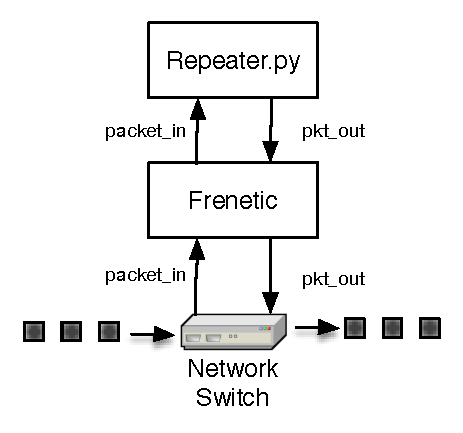
\includegraphics{frenetic_architecture}

\begin{enumerate}
\item At the bottom is your switches and wires.  In our lab setup, Mininet and OpenVSwitch is a substitute for this layer.
\item In the middle is Frenetic.  It talks the OpenFlow protocol to the switches (or to Mininet) -- this is called the Southbound interface.  It also accepts its own language called NetKAT from network applications -- this is called the Northbound interface.
\item At the very top is your network application, which you write in Python.  It defines how packets are dealt with.
\end{enumerate}

We wrote a very simple network application that emulates a network repeater.   
It responds to the \lstinline{packet_in} event coming from the switches through Frenetic when a packet 
arrives at the switch.  
And it sends the \lstinline{pkt_out} message to send the packet back out through Frenetic to the switch.  
Frenetic-vm makes installing and testing all the pieces straightforward. 
When you're done, your network application can be deployed to a real production network.

Obviously you can do much more than just simple repeating with SDN!  
We'll cover that next with some background on OpenFlow and NetKAT, the underlying language of Frenetic. 